\begin{figure*}[t]
\begin{center}
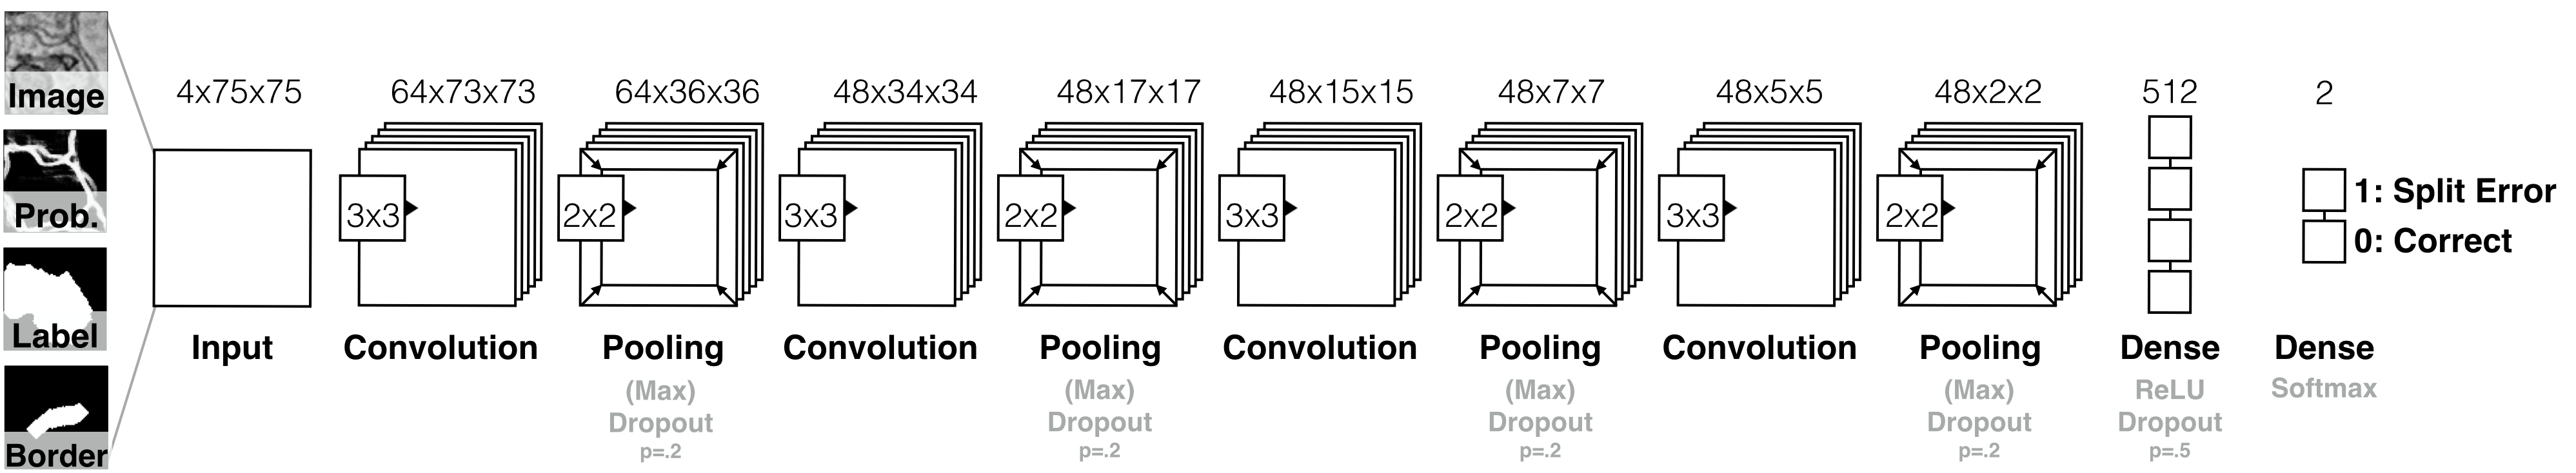
\includegraphics[width=\linewidth]{gfx/architecture.png}
\end{center}
  \vspace{-4mm}
   \caption{We build the guided proofreading classifiers using a traditional CNN architecture. The network is based on four convolutional layers, each followed by max pooling as well as dropout regularization. The 4-channel input patches are rated as either correct splits or as split errors.}
\label{fig:architecture}
\end{figure*}

\section{Related Work}

Proofreading is performed on top of an existing automatic segmentation. First, this section gives an overview of state-of-the-art automatic segmentation methods. Then, we discuss interactive proofreading tools and recent developments in computer-aided proofreading systems.

\textbf{Automatic Segmentation.} Multi-terabyte EM brain volumes require automatic segmentation~\cite{jain2010,Liu2014,NunezIglesias2013Machine,GALA2014}, but can be hard to classify due to ambiguous intercellular space: the 2013 IEEE ISBI neurites 3D segmentation challenge~\cite{isbi_challenge} showed that existing algorithms which learn from expert-segmented training data still exhibit high error rates.

NeuroProof \cite{neuroproof2013} tries to decrease error rates with interactive learning of agglomeration of over-segmentations of images, based on a random forest classifier. Vazquez-Reina \etal~\cite{amelio_segmentation} propose automatic 3D segmentation by taking whole EM volumes into account rather than a per section approach, then solving a fusion problem with a global context. Kaynig \etal~\cite{kaynig10} propose a random forest classifier coupled with an anisotropic smoothing prior in a conditional random field framework with 3D segment fusion. It is also possible to learn segmentation classification features directly from images with CNNs. Ronneberger \etal~\cite{RonnebergerFB15} use a contracting/expanding CNN path architecture to enable precise boundary localization with small amounts of training data. Lee \etal~\cite{lee2015recursive} recursively train very deep networks with 2D and 3D filters to detect boundaries. Bogovic \etal~\cite{BogovicHJ13} learn 3D features, and show even that unsupervised learning can produce better features than hand-designs. Our work was inspired by this paper and we extend the features reported by Bogovic \etal for our guided proofreading classifiers as described in section \ref{sec:methods}.
These approaches make good progress; however, in general, proofreading is required to improve them through generating more ground-truth segmentations. 

\textbf{Interactive Proofreading.} While proofreading is very time consuming, it is fairly easy for humans to perform corrections through splitting and merging segments. One way to perform such corrections is by using expert tools such as Raveler introduced by Chklovskii~\etal~\cite{chklovskii2010, raveler}. This software offers many parameters for tweaking the proofreading process. Created in 2010, Raveler is still used today by professional full-time proofreaders and many similar systems exist as stand-alone products or plugins to existing visualization system,~\eg V3D~\cite{proofreading_bottleneck} or AVIZO~\cite{markus_proofreading}. In contrast to these expert tools, recent works attack the problem of proofreading massive datasets by novices through crowd-sourcing~\cite{saalfeld09,anderson2011,Giuly2013DP2}. A very popular platform is EyeWire presented by Kim \etal~\cite{eyewire_nature}. EyeWire is set up as an online game and participants earn virtual rewards for merging oversegmented labeling to reconstruct the retina cells.
A range of proofreading tools exist in-between expert systems and online games such as Mojo and \textit{Dojo} developed by Haehn \etal~\cite{haehn_dojo_2014,Neuroblocks}. Mojo provides a simple scribble interface for error correction, and Dojo extends this for distributed proofreading via a minimalistic web-based user interface. The authors define requirements for general proofreading tools, and then evaluate the accuracy and speed of Raveler, Mojo, and Dojo through a quantitative user study (Sec. 3 and 4)~\cite{haehn_dojo_2014}. In this paper, we use the Dojo system as a baseline for interactive proofreading and extend the experiment reported by Haehn \etal, where Raveler, Mojo, and Dojo are compared in terms of accuracy and speed.
All interactive proofreading solutions require the user to find potential errors manually which takes the majority of time~\cite{proofreading_bottleneck,haehn_dojo_2014}. Recent works propose computer-aided proofreading systems which help with this visual search task.

%Most relevant methods here use heuristics to analyze the image data to find potential errors. 
\textbf{Computer-aided Proofreading.} To reduce the time spent looking for errors, Plaza proposed \textit{focused proofreading} (FP) ~\cite{focused_proofreading}. His approach finds split errors by analyzing segment size ratios across slices and then offers yes/no questions to correct these errors. Plaza reports that additional processing beyond FP is required to find merge errors. His method is freely available as open source software and is integrated into Raveler. This makes it feasible for us to use FP as a baseline for evaluating guided proofreading as described in section \ref{sec:evaluation}. A similar approach was published by Karimov \etal as guided volume editing~\cite{karimov_guided_volume_editing}. Measuring differences in histogram distributions in image data enables to find potential split and merge errors in the corresponding segmentation. For merge errors, the authors generate possible boundaries using watershed which inspired our approach as described in section \ref{sec:methods}. Guided volume editing was designed to let expert users correct labeled computer-tomography datasets by performing several interactions per correction. While focused proofreading and guided volume editing both use a heuristical approach to analyze the image data, Uzunbas \etal showed that potential labeling errors can be found by considering the merge tree of an automatic segmentation method~\cite{uzunbas}. The authors track uncertainty throughout the automatic labeling by training a conditional random field. This method is really a segmentation technique but it is possible to use the uncertainty information to present potential regions for proofreading. Uzunbas' paper describes a great idea but requires further work to overcome the requirement of isotropic volumes, a property not given for most connectomics datasets. Our approach, guided proofreading, works on isotropic as well as anisotropic data, and finds merge and split errors.